\documentclass[10pt,a4paper]{article}
\usepackage[utf8]{inputenc}
\usepackage{amsmath}
\usepackage{amsfonts}
\usepackage{amssymb}
\usepackage{amsthm}
\usepackage{graphicx}
\usepackage{stmaryrd}
\usepackage{url}
\usepackage{hyperref}
\newtheorem{thm}{Theorem}[section]
\newtheorem{lem}[thm]{Lemma}
\newtheorem{cor}[thm]{Corollary}
\theoremstyle{plain}
\newtheorem{mydef}[thm]{Definition}
\theoremstyle{definition}
\newtheorem{myex}[thm]{Example}
\usepackage[english]{babel}
\newcommand\tab[1][1cm]{\hspace*{#1}}
\usepackage{qtree}
\usepackage{tabularx}

\author{First Draft}
\title{Learning of Safety Controllers using Horn Constraints}

\begin{document}
\maketitle
\begin{abstract}
Infinite-duration two-person games are a popular formalism for synthesizing reactive controllers. In this work, we consider safety games (which arise from safety specifications) and show how safety controllers can be computed using machine learning. At the heart of our approach lies a novel decision tree learning algorithm that learns from Horn constraints and has recently been developed for the verification of concurrent programs. We implement a teacher and show how we can use the Horn learner to synthesize a controller. Furthermore, we show that there is a bounded algorithm that guarantees the learning process to terminate in polynomial time.
\end{abstract}

\section{Introduction}

We are looking to synthesize reactive controllers subject to safety specifications. We model the interaction between system and environment as a two-player safety game over possibly infinite graphs. Thus, the usual approach of fixpoint computation doesn't work on this kind of problems. Instead, we use a a teacher learning setting to learn a controller. The teacher has knowledge about the game and the learner proposes hypothesis about a winning set in the game. 

Based on the ICE learning framework the teacher responds with counterexamples. Those counterexamples can have four different types: positive, negative, existential implication and universal implication counterexamples. We use a decision tree learner for Horn Samples and need to encoded our counterexamples accordingly to fit those requirements. The learning takes place iteratively. In each iteration the learner proposes a hypothesis to the teacher and the teacher responds with either a counterexample or none. The latter meaning that the hypothesis is indeed a winning set. Otherwise the learner incorporates the counterexample in the next iteration of synthesizing a hypothesis.  

One result of this paper is that we can transform a Game Sample that consists of such counterexamples into a Horn Sample that consists of Horn constraints. This allows us to use the already existing Horn learner\cite{d2017horn}. The teacher itself is based on the symbolic computation of counterexamples, used in "An Automaton Learning Approach to Solving Safety Games over Infinite Graphs" \cite{neider2016automaton}. But instead of using automata, we use SMT-solver to compute the counterexamples. This form of computation allows us to avoid exponential blow up by allowing us to not iterate over all possible solution but instead have an symbolic representation of our game.

In detail, we learn a winning set for the controlled system.  With the help of a winning set we can determine a strategy by staying inside the winning set. Once in the winning set the controlled system can force to stay inside this set of vertices. 

The main results of this paper are how to use a decision tree learner for Horn Samples to compute a winning set. A teacher using an SMT-solver to compute the counterexamples needed for the learner and the transformation of the Game Sample that consists of those counterexamples to a Horn Sample. Finally, we show that using our algorithm with the bounded Horn learner is guaranteed to converge.



\section{Overview}
We give an overview of all definitions that will be used during this paper. These include the definition of safety games and horn constraints. One of the first things we have to understand is the notion of data points.
 
We use data points over a domain $D$ to describe points in our graph. Our learner can use Horn constraints to build a tree $\mathcal{T}$, which evaluates data points to a boolean value ($\mathcal{T}:D \to \mathbb{B}$). The learning algorithm constructs a tree using a set of base predicates which evaluate to $true$ or $false$ on data points.
We can see, that a boolean function $f: D \to \mathbb{B}$ induces a valuation $v: D \to {true,false}$, where $x \mapsto_f 1 \iff x\mapsto_v true$
\subsection{Safety Games}

We want to learn winning strategies for safety games, but we have to define first what a safety game is.
We say that a safety game is a infinite duration game over a graph with a countable set of vertices. Safety games are played on an arena $\mathfrak{A} = (V_{0}, V_{1}, E)$, where $V_{0}$ and $V_{1}$ are disjoint and countable sets of vertices and $E$ defines a directed edge relation $E \subseteq V \times V$. We write successor of a set of vertices as $E(X) = \{y \;|\; \exists x \in X : (x,y) \in E\}$.
The initial vertices of a safety game are defined in the following way. $\mathfrak{G} = (\mathfrak{A}, F, I)$, $\mathfrak{A} = (V_{0}, V_{1}, E)$ is an arena, $F \subseteq V$ a set of \textit{safe vertices} and $I \subseteq F$ a set of \textit{initial vertices}. The next thing is to explain how this safety games are played. We have two players, Player 0 and Player 1 and each of them owns a set of vertices. Player 0 owns the vertices that are in $V_{0}$ and Player 1 the vertices in $V_{1}$. The safety game starts when a initial token is placed on one initial vertex $v_{0} \in I$. The player owning the vertex can move the token to one of its successors. Since we are talking about infinite duration games, the process is repeated ad infinitum. This yields a infinite sequence of vertices $v_{0}v_{1}...$ that we call a \textit{play} iff $v_{0} \in I$ and $(v_{i}, v_{i+1}) \in E$ for all $i \in \mathbb{N}$. A play is \textit{winning} for Player 0 if $v_{i} \in F$ for all $i \in \mathbb{N}$. Otherwise the play is \textit{winning} for Player 1.

A strategy for Player $\sigma$, $\sigma \in \{0,1\}$, is a mapping $f_{\sigma} : V*V_{\sigma} \to V$. A winning strategy yields a winning play for any play that is created using the strategy. We can get a winning strategy if you look at the \textit{winning set} of a safety game which is defined as follows.
\paragraph*{Winning set} For a safety game $\mathfrak{G} = (\mathfrak{A}, F, i)$ over the arena $\mathfrak{A} = (V_{0}, V_{1}, E)$, a winning set is a set $W \subseteq V$ satisfying
\begin{enumerate}
\item $I \subseteq W$
\item $W \subseteq F$
\item $E(\{v\}) \cap W \neq \emptyset$ for all $v \in W \cap V_{0}$
\item $E(\{v\}) \subseteq W$ for all $v \in W \cap V_{0}$
\end{enumerate}

A winning strategy for Player 0 would be to move inside the winning set. This can be proven with a induction over the length of plays. Since we want to use binary decision diagrams for the learning process, we need construct BDDs that represent the sets $I$, $W$, and $F$.  

\subsection{Teacher and learner interaction}

In this section we want to explain how the teacher and the learner interact with each other.
Since we want to learn safety games, we need to compute winnings sets. Winnings sets have the above defined properties. We will follow the ICE-learning approach by learning with counterexamples, meaning if one of the properties is unsatisfied we can generate one counterexample. We can give positive counterexamples if property $I \subseteq W$ is unsatisfied and a negative counterexample if $W \subseteq F$ is unsatisfied.
For the third property we can give existential counterexamples ($ x \to (x_1 \vee  ... \vee x_k)$) and for the fourth we can give universal counterexamples ($ x\to (x_1 \wedge ... \wedge x_k)$). We will show later that it is possible to transform those counterexamples into horn constraints.

The teacher has knowledge about the safety game and can verify winning sets that the learner proposes. The teacher gives the learner counterexamples if the proposed winning set is wrong. 
The learner makes a conjecture about the winning set using the counterexamples given by the teacher. Then he gives the teacher his constructed winning set.
The interaction between teacher and learner takes place in rounds. In each round the learner makes a new conjecture and the teacher either accepts it or gives the learner a counterexample for his conjecture.

The counterexamples of the teacher have the form mentioned in the construction, so we can transform them to horn constraints and build a binary decision tree with the help of the constraints. This binary decision tree describes our winning set. Afterwards, the teacher has to check if the tree fulfills the properties.


\paragraph*{arena} $\mathfrak{A} = (V_{0}, V_{1}, E)$, where $V_{0}$ and $V_{1}$ are disjoint and countable sets of vertices and $E$ defines a directed edge relation $E \subseteq V \times V$
\paragraph*{safety game} $\mathfrak{G} = (\mathfrak{A}, F, i)$, $\mathfrak{A} = (V_{0}, V_{1}, E)$ is an arena, $F \subseteq V$ a set of \textit{safe vertices} and $I \subseteq F$ a set of \textit{initial vertices}
\paragraph*{play} $v_{0}v_{1}...$ is called a \textit{play} iff $v_{0} \in I$ and $(v_{i}, v_{i+1}) \in E$ for all $i \in \mathbb{N}$
\paragraph*{strategy}A strategy for Player $\sigma$, $\sigma \in \{0,1\}$, is a mapping $f_{\sigma} : V*V_{\sigma} \to V$
\paragraph*{winning play} A play is \textit{winning} for Player 0 if $v_{i} \in F$ for all $i \in \mathbb{N}$
\paragraph*{winning strategy} 
A strategy for Player $\sigma$, $\sigma \in \{0,1\}$, is a mapping $f_{\sigma} : V*V_{\sigma} \to V$
\paragraph*{winning set} For a safety game $\mathfrak{G} = (\mathfrak{A}, F, i)$ over the arena $\mathfrak{A} = (V_{0}, V_{1}, E)$, a winning set is a set $W \subseteq V$ satisfying
\begin{enumerate}
\item $I \subseteq W$
\item $W \subseteq F$
\item $E(\{v\}) \cap W \neq \emptyset$ for all $v \in W \cap V_{0}$
\item $E(\{v\}) \subseteq W$ for all $v \in W \cap V_{0}$
\end{enumerate}
\begin{mydef}
A \emph{Horn Sample} is a set $S = (X,C)$, where $X$ is a set of positive and negative data points and $C$ is a set consisting of Horn constraints over $X$. Those formulas have the following structure:
\begin{enumerate}
\item $true \to x$
\item $x \to false$
\item $x_1 \wedge...\wedge x_k \to x $
\end{enumerate}
\end{mydef}
\begin{mydef}
A \emph{Game Sample} is a set $S = (X,C)$, where $X$ is a set of positive and negative data points and $C$ is a set of formulas over $X$. Those formulas have the following structure:
\begin{enumerate}
\item $true \to x$
\item $x \to false$
\item $x \to x_1 \vee  ... \vee x_k$
\item $x \to x_1 \wedge ... \wedge x_k$ 
\end{enumerate}
\end{mydef}

\begin{mydef}
A Horn Sample is \emph{valid} $\iff $ there is a valuation $v$ such that $v \vDash C$.
\end{mydef}
\begin{mydef}
A Game Sample is \emph{valid} $\iff $ there is a valuation $v$ such that $v \vDash C$.
\end{mydef}

\subsection{Horn constraints and how to use them with data points}
We have a set of formulas $C$ over a set of data points $X \subseteq D$ that are Horn constraints.
A Horn clause (or a Horn constraint) over $X$ is a disjunction of literals over $X$ with at most one positive literal.
These are not boolean formulas since the formulas go over data points. We call $S :=(X,C)$ a Game sample, where $C = \{c_1,..,c_m\}$ is a set of formulas that are Horn constraints, but instead of variables we have data points, and $D(C) := \{D(c)|c \in C\}$ is a set of data points that appear in the formulas. But we want to evaluate Horn constraints over boolean variables. To do this we need a new Horn sample $S' = (X',C')$, but this time we have Horn constraints over boolean variables. To get this sample we need define a bijective function $v: D(C) \to X';d \mapsto x_d$ that maps our data points to variables that we use in our Horn constraints. Additionally, $C'$ has the same Horn constraints like $C$, but every data point is replaced with its variable. We can now define a valuation for $X'$, $v_\mathcal{T}: X' \to \mathbb{B};x_d \mapsto t(v^{-1}(x_{d}))$. We say a Horn sample $S = (X,C)$ over boolean variables is consistent with a tree $\mathcal{T}$ if and only if $v_{\mathcal{T}} \vDash \bigwedge_{c \in C} c$.
\paragraph*{existential counter example} $x \to \bigvee_{i} x_i$
\paragraph*{universal counter example} $ x \to \bigwedge_{i} x_i$
\paragraph*{data points} elements of a abstract domain $\mathbb{D}$ for example vectors of integers
$\vec{x_1} = [3,4,5], \vec{x_2} = [4,2,7]$.$a_1$ describes the first entry of the vector $a_2$ the second and $a_3$ the third entry of the vector.
\paragraph*{valuation} a valuation $v$ for a set of predicates is a function $v: X \to \{true,false\}$
\paragraph*{decision tree} binary trees whose internal nodes are labeled with predicates and leafs are either true or false. (definition in the paper)
\paragraph*{formula of a decision tree}
\begin{equation}\label{Formula of a decision tree}
\psi_\mathcal{T} =\bigvee_{\pi \in \Pi_{true}} (\bigwedge_{\rho \in \Pi} \rho)
\end{equation}

\paragraph*{evaluation of data points over a decision tree} Given a set of data points X, a decision tree can evaluate them to $true$ or $false$.
\paragraph*{Example for a valuation over a decision tree.}
\begin{equation*}
\begin{split}
 D &:= \{\vec{x_1},\vec{x_2}\}, \vec{x_1} = [3,4,5], \vec{x_2} = [4,2,7]\\
 \mathcal{P} &:= \{p_1,p_2\}, p_1 := a_1 \leq 3 \wedge a_2 \leq 4 \wedge a_3 \leq 5, p_2 :=a_1 \leq 6 \wedge a_2 \leq 7 \wedge a_3 \leq 8 \\
 p_1(\vec{x_1}) &= true, p_1(\vec{x_2}) = false\\
 p_2(\vec{x_1}) &= true, p_2(\vec{x_2}) = true
\end{split}
\end{equation*}
Assume following tree constructed by the learner:
\Tree [.p_1 [.p_2 [.true ] [.true ] ].p_2 [.false ] ].p_1

A valuation of $\vec{x_1}$ and $\vec{x_2}$ would look like this:
\begin{equation*}
\begin{split}
v_\mathcal{T}(\vec{x_1}) &= p_1(\vec{x_1}) \wedge p_2(\vec{x_1}) \vee p_1(\vec{x_1}) \wedge \lnot p_2(\vec{x_1}) = true\\
v_\mathcal{T}(\vec{x_2}) &= p_1(\vec{x_2}) \wedge p_2(\vec{x_2}) \vee p_1(\vec{x_2}) \wedge \lnot p_2(\vec{x_2}) = false 
\end{split}
\end{equation*}
\paragraph*{Horn constraints} A Horn clause (or a Horn constraint) over $X$ is a disjunction of literals over $X$ with at most one positive literal.
\paragraph*{consistency} A decision Tree $\mathcal{T}$ is consistent with Horn constraints $C$ over data points $X$ if 
$v_\mathcal{T} \vDash \bigwedge C$
\begin{mydef}
A \emph{Horn Sample} is a set $S = (X,C)$, where $X$ is a set of positive and negative data points and $C$ is a set consisting of Horn constraints over $X$. Those formulas have the following structure:
\begin{enumerate}
\item $true \to x$
\item $x \to false$
\item $x_1 \wedge...\wedge x_k \to x $
\end{enumerate}
\end{mydef}
\begin{mydef}
A \emph{Game Sample} is a set $S = (X,C)$, where $X$ is a set of positive and negative data points and $C$ is a set of formulas over $X$. Those formulas have the following structure:
\begin{enumerate}
\item $true \to x$
\item $x \to false$
\item $x \to x_1 \vee  ... \vee x_k$
\item $x \to x_1 \wedge ... \wedge x_k$ 
\end{enumerate}
\end{mydef}

\begin{mydef}
A Horn Sample is \emph{valid} $\iff $ there is a valuation $v$ such that $v \vDash C$.
\end{mydef}
\begin{mydef}
A Game Sample is \emph{valid} $\iff $ there is a valuation $v$ such that $v \vDash C$.
\end{mydef}

\section{Transformation from Game Sample to Horn Sample}
Let $C$ be a set of formulas over a set of variables $X$. These formulas are of the following forms:
\begin{enumerate}
\item $true \to x$
\item $x \to false$
\item $ x \to (x_1 \vee  ... \vee x_k)$
\item $ x\to (x_1 \wedge ... \wedge x_k)$
\end{enumerate}

Define for a valuation $v$ over $X$ a new valuation $v': X \to \mathbb{B}; x \to 1-v(x)$.
Define a set of horn constraints $C'$. Add a new formula to $C'$ for every formula in $C$:
\begin{enumerate}
\item $\forall (true \to x\in C)$ add $(x \to false)$ to $C'$
\item $\forall (x \to false\in C)$ add $(true \to x)$ to $C'$
\item $\forall (x \to (x_1 \vee  ... \vee x_k)\in C)$ add $ ((x_1 \wedge...\wedge x_k) \to x)$ to $C'$
\item $\forall (x \to (x_1 \wedge ... \wedge x_k)\in C)$ add a set of formulas $\{x_i \to x | i \in \{1,...,k\}\}$ to $C'$.
\end{enumerate}
We can  see that $C'$ is a set of Horn constraints.

\begin{lem}
\textit{Let $v$ be a valuation for a set of formulas $C$ like in the construction above. Let $v'$ be the valuation and $C'$ a set of horn constraints we get by applying the construction. Then:}
\end{lem}
\[v \vDash C \iff v' \vDash C'\]
\begin{proof} $\\ $
Let $v$ be a valuation for $C$. If $v \vDash C$ then $v \vDash \bigwedge_{c \in C} c$ and $\forall c \in C : v \vDash c$. Therefore, it is enough to perform a case analysis for each formula $c \in C$. We do this by applying the described construction above to $v$ and $C$:
\begin{enumerate}
\item We apply the construction to formulas of the form $c:= true \to x$ and get $c':= x\to false$:
\begin{equation*}
\begin{split}
v & \vDash c \iff v \vDash x \iff v' \nvDash x \iff v' \vDash c'
\end{split}
\end{equation*}

\item We apply the construction to formulas of the form $c:= x \to false$ and get $c':= true \to x$:
\begin{equation*}
\begin{split}
v & \vDash c \iff v \nvDash x \iff v' \vDash x \iff v' \vDash c'
\end{split}
\end{equation*}
%(v  \vDash x) \wedge
\item We apply the construction to formulas of the form $c:=(x \to (x_1 \vee  ... \vee x_k))$ and get $c':= (x_1 \wedge...\wedge x_k) \to x)$:
\begin{equation*}
\begin{split}
v &\vDash c \iff (\exists i\in \{1..k\}: v \vDash x_i) \vee (v \nvDash x) \\
\iff (v' &\vDash x) \vee ((\exists i\in \{1..k\}: v' \nvDash x_i)) \iff v' \vDash c'
\end{split}
\end{equation*}
\item We apply the construction to formulas of the form $c  := x \to (x_1 \wedge ... \wedge x_k)$ and get $c':=\{x_i \to x | i \in \{1,...,k\}\}$:
\begin{equation*}
\begin{split}
v  \vDash c \iff (\forall i\in \{1..k\}: &v \vDash x_i) \vee (v \nvDash x)\\
\iff (v' \vDash x) \vee ((\forall &i \in  \{1..k\}: v' \nvDash x_i)) \\
\iff (\forall i\in \{1..k\}:& v' \vDash  x_i \to x) \iff v' \vDash c'
\end{split}
\end{equation*}
\end{enumerate}
Summarizing the case analysis we can see that if we take any formula in $c \in C$ and transform it into a formula  $c' \in C'$ we get that $v \vDash c \iff v' \vDash c'$ and therefore $v \vDash C \iff v' \vDash C'$ for any valuation $v$.

\end{proof}
\begin{cor} \label{Korollar}

A formula $\psi$ is consistent with a Game Sample if and only if it is consistent with the corresponding Horn Sample.
\end{cor}
\begin{proof}
Let $\psi $ be a formula that is consistent with the Game Sample $S_{Game}$. Now we have to perform a case analysis again for each formula $c \in C_{Game}$.
\begin{enumerate}
\item
\begin{equation*}
\begin{split}
x \to x_1 \vee &\dots \vee x_n \; is \; consistent \; with \; \psi \\
\iff &(\exists i \in \{1,\dots,n\}: x_i \vDash \psi) \vee (x \nvDash \psi) \\
\iff &(x' \vDash \psi) \vee ((\exists i\in \{1..n\}: x_i' \nvDash \psi)) \\
\iff &x_1' \wedge \dots \wedge x_n' \to x' \; is \; consistent \; with \; \psi 
\end{split}
\end{equation*}
\item The rest of the cases are similarly proven.
\end{enumerate}
\end{proof}

\section{Bounded Decision Tree Learner for Horn Samples}
\begin{thm} \label{Theorem1}
If the input set of points X is separable and the input Horn Constraints are satisfiable, then the Learner always terminates with a decision tree consistent with the Horn sample (X,C).\cite{d2017horn}
\end{thm}

\begin{mydef}
Given an Horn sample $S = (X,C)$. Define the equivalence class $\equiv_m$ m on X: $\\ \\ $ 

$s \equiv_m s'$ $\iff$ there is no predicate of the form $a_i \leq$ $c$ with $|c| \leq$ $m \\ \tab \tab \tab \tab $ that separates $s$ and $s'$.
\end{mydef}

\begin{mydef}
We can augment a sample $S = (X,C)$ to obtain a \emph{m-augmented Horn Sample of S}, denoted by $S \oplus m$. To obtain $S \oplus m$, we first construct the set $E = \{(s,s')\;|\; s \equiv_m s'\}$ and add it to a our Horn Constraints, $(X,C \cup E)$.
\end{mydef}

\begin{thm} \label{Horn Theorem}
Let $S$ be an Horn Sample. Then the following holds:
\begin{enumerate}
\item If $S \oplus m$ is not valid, then there is \emph{no Boolean formula with absolute maximum threshold m} that is consistent with $S$. In the overall learning loop, we would increment $m$ in this case and restart learning from $S$.

\item If $S \oplus m$ is valid, then calling our Decision Tree Learner for Horn Samples on $S \oplus m$ while restricting it to predicates that use thresholds with absolute values at most $m$ is \emph{guaranteed to terminate and return a tree that is consistent with S}. 
\end{enumerate}
\end{thm}
% anstatt s_i in S^+ usw. Learner findet kein assignment sodass, die horn klauseln erfüllbar sind? neeee
\begin{proof} $\\ $ 
\begin{enumerate}
\item Assume $S \oplus m$ is not valid. This means the Horn Solver returns with an unsat. Now for the sake of contradiction assume that there is a Boolean formula $f$ with absolute maximum threshold m that is consistent with S. Thus, $f$ satisfies all the new horn constraints added and consequently $S \oplus m$. Thus calling our Horn Solver on $S \oplus m$ should have returned with a boolean function $f'$ which assigns the values in $X$ according to f which is a contradiction to our Horn Solver returning unsat.

\item Assume now that $S \oplus m$ is valid.  We need to show that the input set of points is separable. For this assume that our bounded Decision Tree Learner for Horn Samples processes a node with the sample of $S \oplus m$. Moreover, assume that we can't find a split with threshold $|c| \leq m$. We know that the data points we want to split can't be pure. Otherwise, we have a split which assigns them all to one side. Thus, there are three different cases that can happen, two of those are analogous.
\begin{enumerate}
\item We have at least one positively classified data point p and at least one negatively classified data point n. Since we can't separate those two points, we know that they are in the same m-equivalence class. Thus, $(p,n)$ is a horn constraint in $S \oplus m$. This means our Horn Solver should have returned with unsat, since $(p,n)$ is an unsatisfiable horn constraint.

\item We have no negatively classified data points. Thus, we only have positively classified data points and unclassified data points. Since those points are inseparable, they are all in the same m-equivalence class. This means that they all have to have the same classification which is positive, making a split possible. This is a contradiction to our assumption that we can't separate those data points.

\item We have no positively classified data points. This is analogous to case (b).
\end{enumerate}

Furthermore, if $S \oplus m$ is valid, then there is a valuation that satisfies $C$.

Now, we have that the input set of points is separable and that $S \oplus m$ is valid and can use Theorem \ref{Theorem1} to get that the Learner always terminates with a decision tree consistent with the Horn sample $(X,C)$.
\end{enumerate}
\end{proof}

\begin{thm}
Let $S_{Game}$ be a Game Sample. Then the following holds:
\begin{enumerate}
\item If $S \oplus m$ is not valid, then there is \emph{no Boolean formula with absolute maximum threshold m} that is consistent with $S$. In the overall learning loop, we would increment $m$ in this case and restart learning from $S$.

\item If $S \oplus m$ is valid, then calling our Decision Tree Learner for Horn Samples on $S \oplus m$ while restricting it to predicates that use thresholds with absolute values at most $m$ is \emph{guaranteed to terminate and return a tree that is consistent with S}. 
\end{enumerate}
\end{thm}
\begin{proof} $\\ $
\begin{enumerate}
\item $S_{Game} \oplus m$ not valid $\Rightarrow$ there is no valuation $v$ such that $v \vDash C$ $\overset{Lemma \;\ref{lemma}} \Rightarrow $ there is no valuation $v'$ for the Horn Sample $S_{Horn} \oplus m$. $\Rightarrow$ $S_{Horn} \oplus m$ is not valid $\overset{Theorem \;\ref{Horn Theorem}}\Rightarrow$ there is no Boolean formula with maximum threshold m that is consistent with $S_{Horn}$

Assume there exists a Boolean formula $f'$ with maximum threshold m such that $f'$ is consistent with $S_{Game}$. With Corollary \ref{Korollar} we know that $f'$ is also consistent with $S_{Horn}$. Thus, we found a Boolean formula with maximum threshold m that is consistent with $S_{Horn}$ which is a contradiction to $S_{Game} \oplus m$ being not valid.

\item $S_{Game} \oplus m$ is valid $\overset{Lemma \;\ref{lemma}}\Rightarrow$ $S_{Horn} \oplus m$ is valid $\overset{Theorem \; \ref{Horn Theorem}} \Rightarrow$ our Learner for Horn Samples returns with a tree that is consistent with $S_{Horn}$, this tree encodes a Boolean formula that is consistent with $S_{Horn}$ $\overset{Corollary\; \ref{Korollar}}\Rightarrow$ this tree is also consistent with $S_{Game}$
\end{enumerate}
\end{proof}
\newpage
\section{Experiments}

\begin{table}[h]
 \caption{Results of the Experiments}
\begin{tabularx}{\textwidth}{p{0.1\textwidth}p{0.1\textwidth} p{0.1\textwidth} p{0.1\textwidth}p{0.1\textwidth} p{0.1\textwidth} p{0.1\textwidth} p{0.08\textwidth}}
\hline
& \multicolumn{7}{c}{Horn Learner}\\ \hline
Game & Time in s & Iter.& Size & $|Pos|$ & $|Neg|$ & $|Ex|$ & $|Uni|$ \\ \hline
Diagonal & 4.769 & 25 & 6 & 11 & 7 & 4 & 2 \\ 
Evasion & 5.1 & 16 & 4 & 1 & 4 & 7 & 3 \\ 
Follow & 44.097 & 181 & 14 & 1 & 129 & 32 & 18 \\ 
Program-repair & 1.2 & 14 & 11 & 1 & 2 & 10 & 0 \\
Laufband & 0.982 & 5 & 3 & 1 & 1 & 1 & 1 \\ 
Quadrat 3x3 & 6.2 & 61 & 13 & 1 & 18 & 19 & 22 \\
Quadrat 5x5 & 4.195 & 41 & 16 & 1 & 13 & 16 & 10 \\
Multitank 3 & 10.7 & 115& 12 & 1 & 82 & 10 & 21 \\

\end{tabularx}
 \label{tab:TESTS} 
\end{table}
\newpage
\section{Conclusion}
\newpage
\section{Appendix}
\subsection{Game examples}
\begin{figure}[h] \label{Laufband}
  \caption{In this example we have a robot moving on an infinite, discrete one-dimensional grid. Two players can control the robot, Player 0 and Player 1. The goal of Player 0 is to let the robot stay in the safe zone, the goal of Player 1 is to move the robot out of it. Both player take turns moving the robot, moving it at most one field in one direction.
.}
  \centering
    {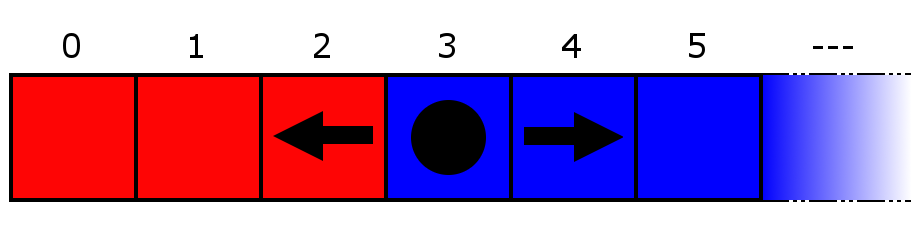
\includegraphics[width=8.0cm]{laufband.png}} 

\end{figure}


\begin{figure}[h]\label{Wassertank}
  \caption{Here we have a water tank and two players. This example works similiar to figure above, but this time the safe zone is limited by two sides since a water tank has only a finite capacity and we don't want the tank to run out of water.
}
  \centering
    {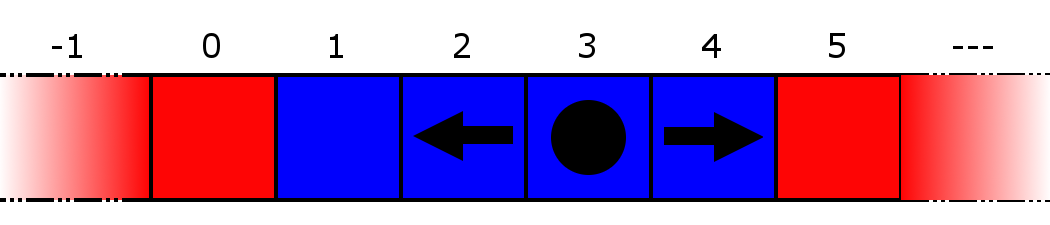
\includegraphics[width=8.0cm]{wasser_tank.png}} 
\end{figure}

\begin{figure}
  \caption{Consider a robot on an infinite two-dimensional grid with two players playing against each other. Both player can move the robot in an arbitrary direction by at most one field. Player 0 tries to keep the robot in a safe square, while Player 1 tries to move the robot out of the square.
}
  \centering
    {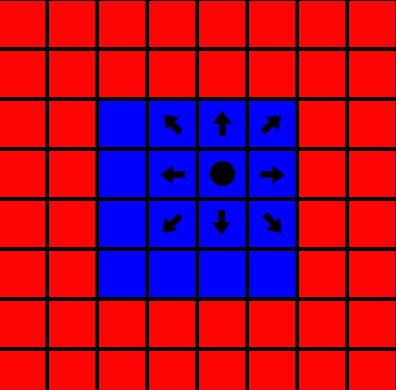
\includegraphics[width=8.0cm]{quadrat.png}} 
\end{figure}


\begin{figure}
  \caption{This example works like the water tank example, played with multiple tanks. Each player can control the tank in its turn and can decide to either fill the tank or empty the tank by one unit.}
  \centering
    {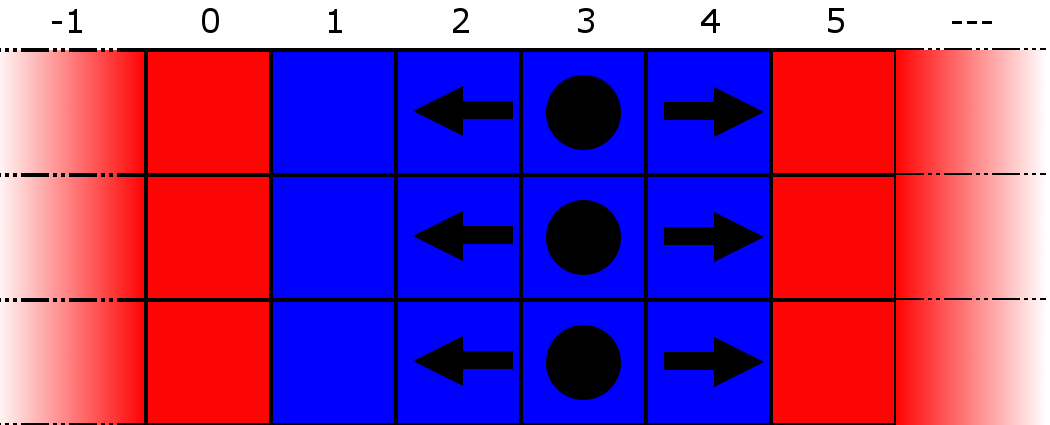
\includegraphics[width=8.0cm]{multi_wasser_tank.png}} 
\end{figure}






\begin{figure}
  \caption{In this example we have an infinite, discrete two-dimensional grid that is limited by two straight lines. Both player can move the robot in an arbitrary direction. Player 0 wins if the robot stays within the area limited by the straight lines. Player 1 wins if the robot moves out of it.}
  \centering
    {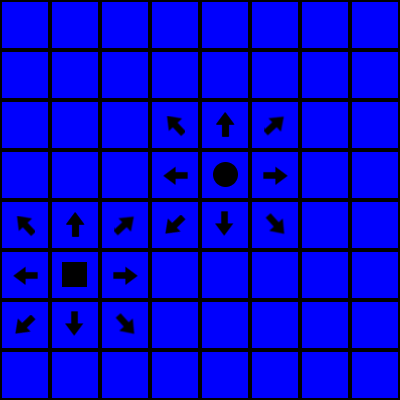
\includegraphics[width=8.0cm]{catch.png}} 
\end{figure}

\begin{figure}
  \caption{We have two robots moving in an infinite, discrete two-dimensional grid. Player 0's objective is to avoid being caught by Player 1.
}
  \centering
    {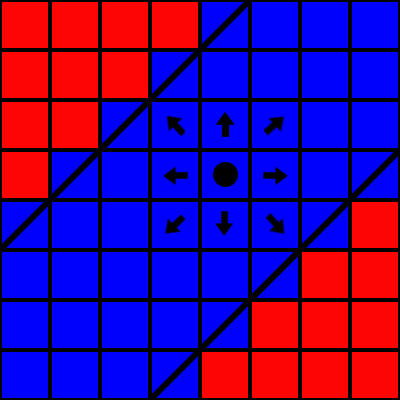
\includegraphics[width=8.0cm]{zwei_geraden.png}} 
\end{figure}
\newpage
\bibliographystyle{plain}
\bibliography{lib}
\end{document}